\documentclass[10pt,a4paper]{article}
\usepackage[utf8]{inputenc}
\usepackage[italian]{babel}
\usepackage{amsmath}
\usepackage{amsfonts}
\usepackage{amssymb}
\usepackage{graphicx}
\usepackage[left=2cm,right=2cm,top=2cm,bottom=2cm]{geometry}
\newcommand{\rem}[1]{[\emph{#1}]}
\newcommand{\exn}{\phantom{xxx}}
\renewcommand{\thesubsection}{\thesection.\alph{subsection}}  %% use 1.a numbering

\author{Gruppo 23M \\ Alessandro Costanzo Ciano}
\title{Es06: Oscillatore a ponte di Wien}
\begin{document}
\date{5 dicembre 2023}
\maketitle


\section*{Scopo dell'~esperienza}
Realizzare e studiare un oscillatore sinusoidale a ponte di Wien con un operazionale TL081 alimentato a +5V e -5V.
%
%

%%%%%%%%%%%%%%%%%%%%%%%%%%%%%%%%%%%%%%%%%%%%%%%%%%%%%%
\section{Misura del loop-gain}

Come prima cosa è stato montato il circuito in figura \ref{fig:circuitoloopgain}, misurando resitenze e capacità, che risultano: \\
$R_1 = (9.93+-0.08)$ kOhm, $R_2 = (9.89+-0.08)$ kOhm, $R_3 = (9.98+-0.08)$ kOhm, $R_4 = (9.91+-0.08)$ kOhm, $C_1 = (10.0+-0.4)$ nF, $C_2 = (10.3+-0.4)$ nF.\\
Per tutte queste l'errore è dato dalla somma in quadratura degli errori errori di scala e di conversione analogico-digitale.

La resistenza massima del trimmer risulta $R_T =  (9.28+-0.08)$ kOhm, mentre le due resistenze che lo compongono, misurate separatamente, risultano complementari ($R_{T1} =  (5.53+-0.05)$ kOhm e $R_{T2} =  (3.7+-0.03)$ kOhm)

\begin{figure}[h]
    \begin{center}
    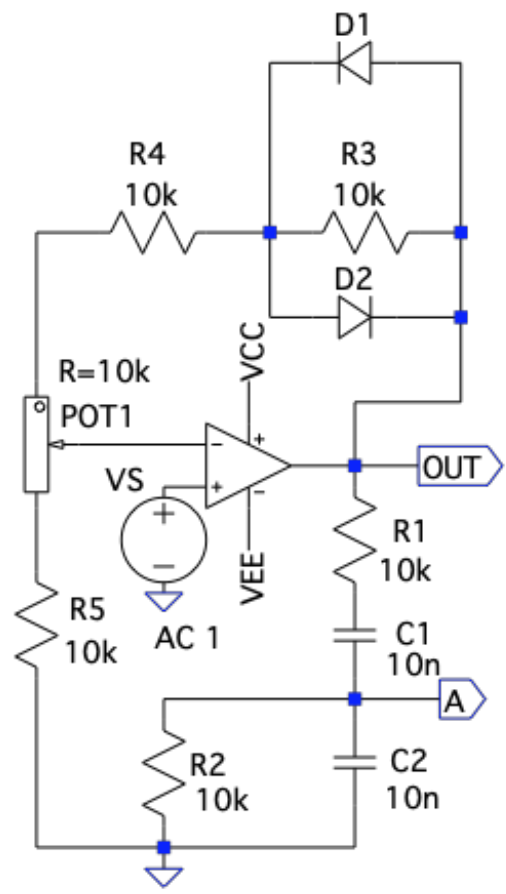
\includegraphics[width=0.4\linewidth]{circuitoloopgain.png}
    \caption{\small Circuito per la misura del loop-gain.}
    \label{fig:circuitoloopgain}
    \end{center}
\end{figure}

\subsection{Regolazione del guadagno dell'amplificatore e studio della
dipendenza dalla frequenza del loop gain $\beta A_V$}

Inviando in $V_S$ un segnale sinusoidale di frequenza 1 kHz ed
ampiezza 500 mV si osservare un'ampiezza di $V_{OUT}$
dipendente dalla posizione del potenziometro. Il
guadagno $A_V = V_{OUT}/V_S$ con il trimmer ad inizio e fine
corsa risulta rispettivamente $A_1 =  3.758+-0.023$ e $A_2 =  2.036+-0.021$ in buon accordo con la previsione di 
\begin{align*}
    A_1 = 1+\dfrac{R_4+R_3+R_T}{R_5}=3.941 +- 0.028
\end{align*}
e di 
\begin{align*}
    A_2 = 1+\dfrac{R_4+R_3}{R_T+R_5} = 2.036+-0.009
\end{align*}
Si osserva che in particolare la leggera discrepanza di $A_1$ potrebbe essere dovuta al raggiungimento della conduzione dei diodi.


Regolata la posizione del trimmer fino ad osservare $A_V = 3$, utilizzando la funzione Network Analyzer di Waveforms
è stata misurata la funzione di trasferimento, del loop-gain $\beta AV = V_A/V_S$ tra 100Hz e 100kHz, avendo fissato l'ampiezza in ingresso a 500
mV (figura \ref{fig:plotbode1}).

\begin{figure}[h]
    \begin{center}
    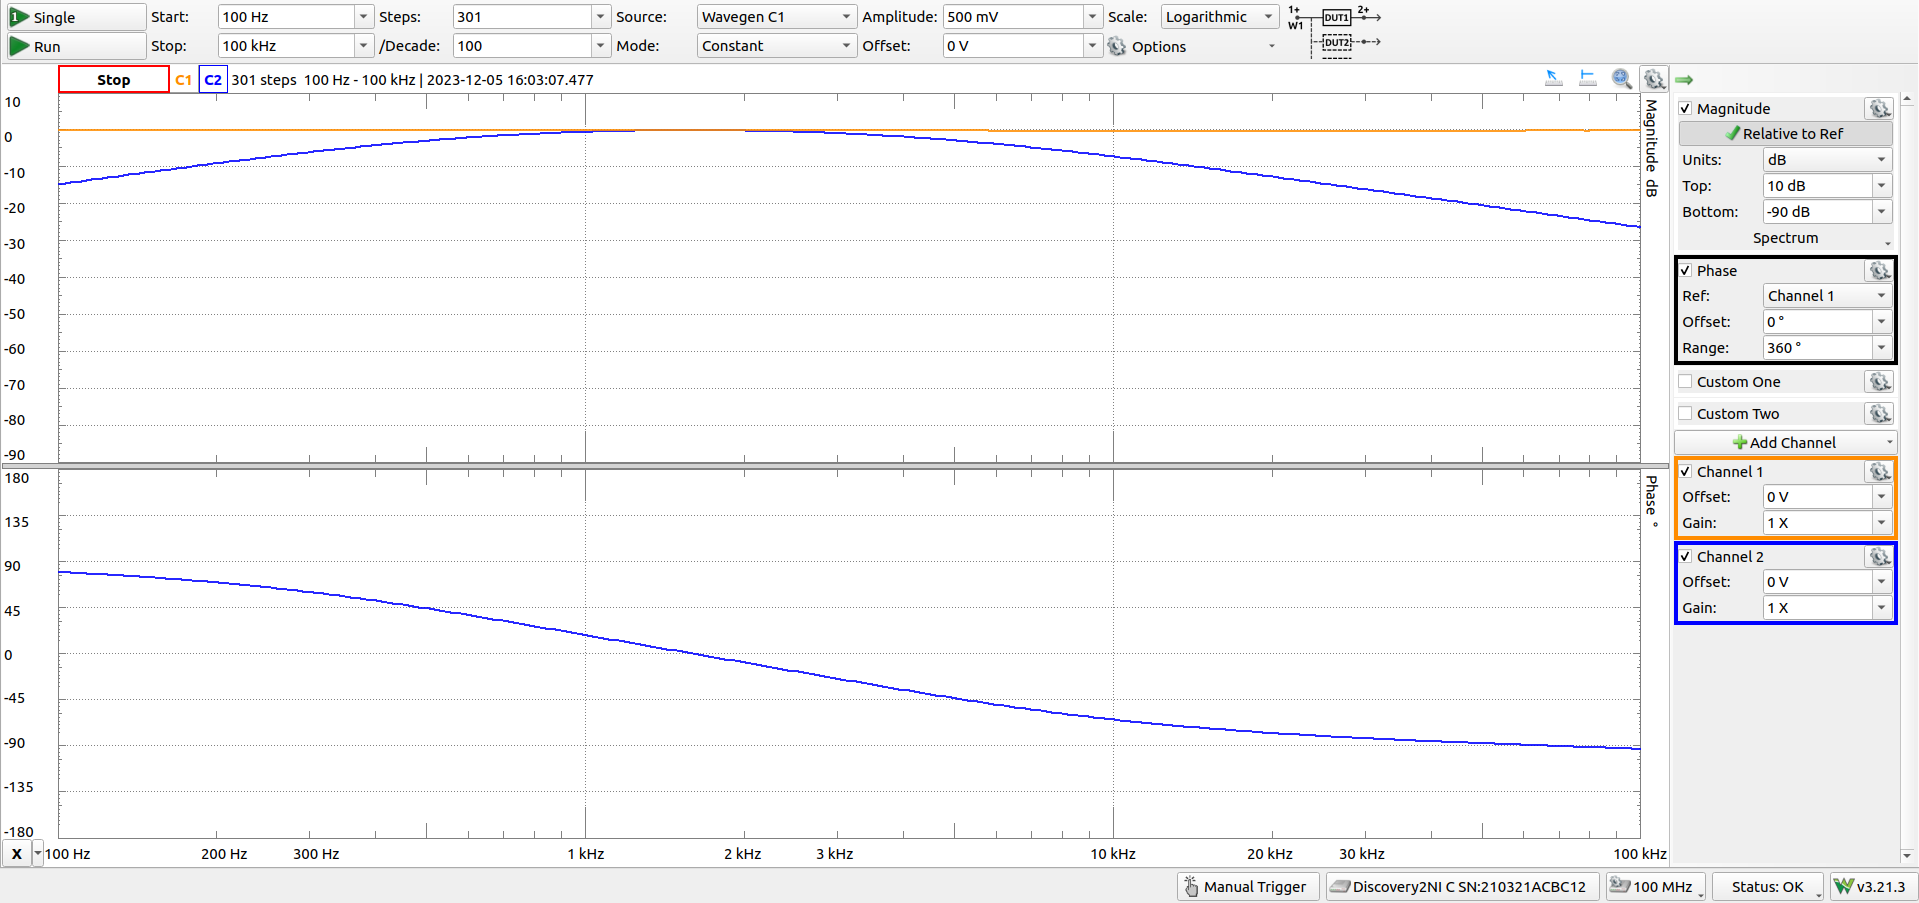
\includegraphics[width=0.7\linewidth]{plotbode1.png}
    \caption{\small Plot di Bode.}
    \label{fig:plotbode1}
    \end{center}
\end{figure}

La frequenza alla quale lo sfasamento si
annulla risulta  $f_0 = (1.6 +- 1) kHz$, con un errore stimato valutando la semiampiezza dell'intervallo intorno al valore misurato per cui non erano apprezzabili variazioni (considerando gli errori di natura diversa trascurabili rispetto a questo).
Esso risulta in accordo con quello atteso $f_0 = 1/(2\pi R_1 C_1)= (1.61+-0.07)$ kHz. Inviando un'onda $V_S$ di 1.6 kHz è statto effettivamente ottenuto $\beta A = 0.986+-0.020$, copatibile con 1. Dunque a tale frquenza è effettivamente soddisfatta la condizione di Barkhausen.
Analizzando il plot di Nyquist (figura \ref{fig:Nyquist1}), è verificabile che il plot sia una circonferenza di centro (1/2, 0) e raggio
1/2.

\begin{figure}[h]
    \begin{center}
    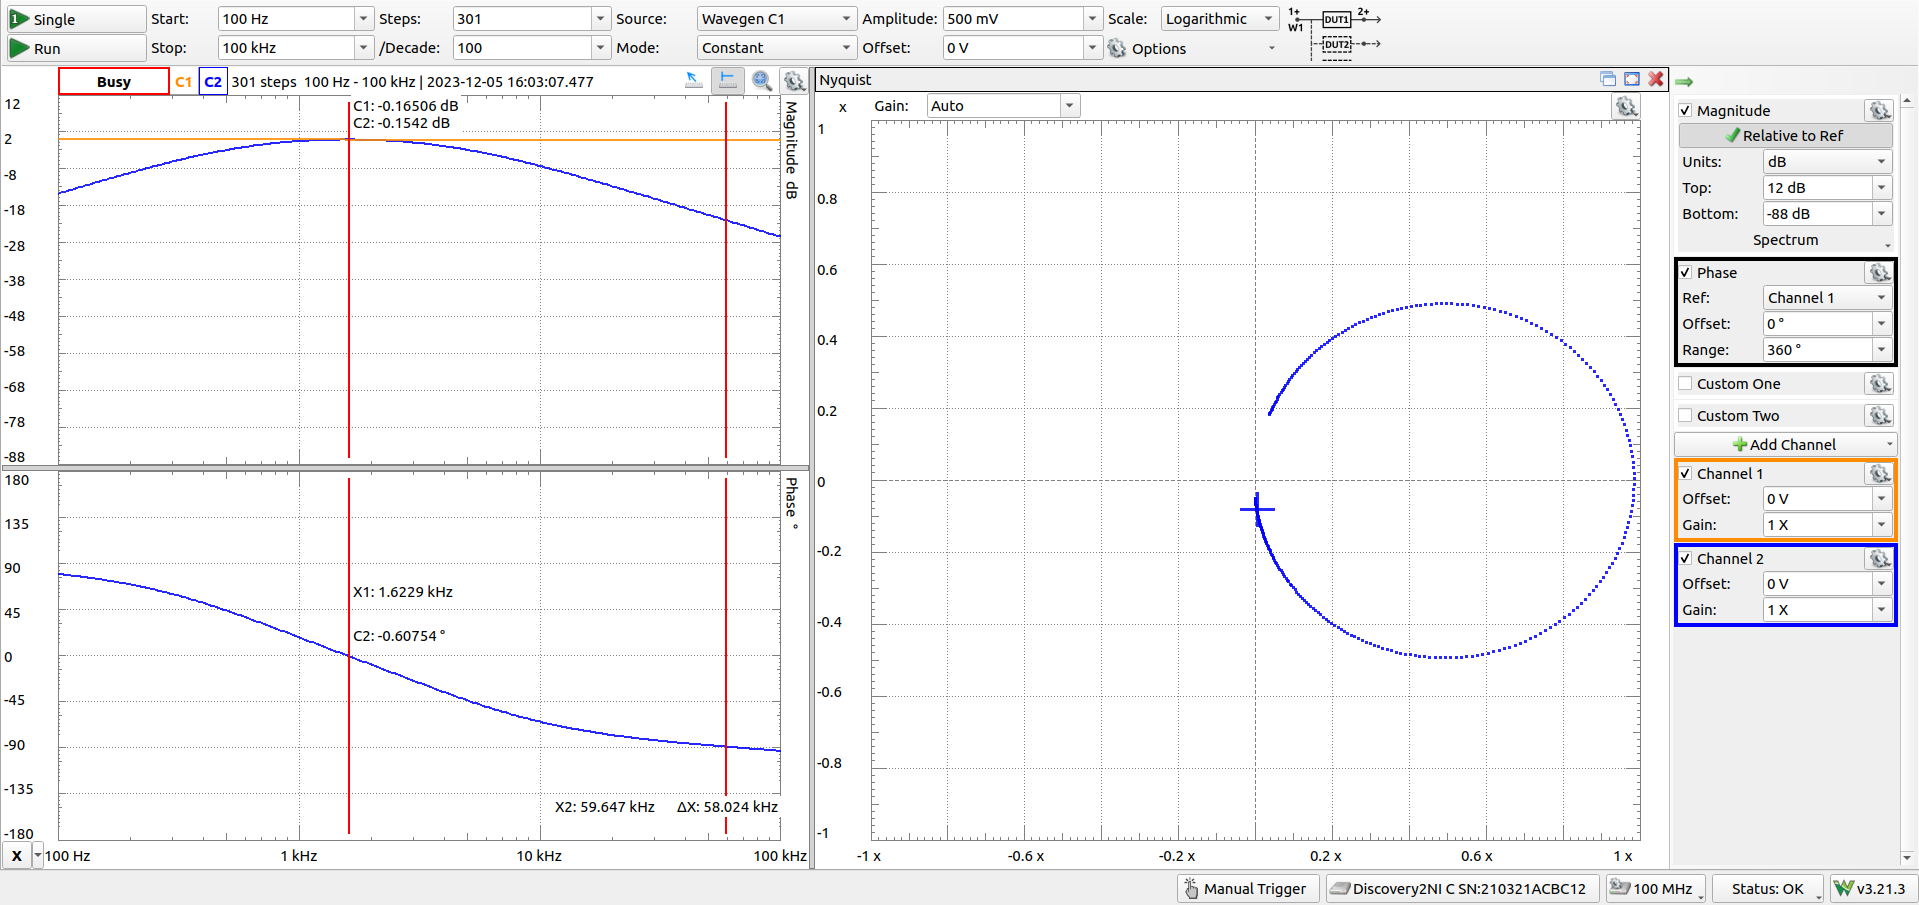
\includegraphics[width=0.7\linewidth]{Nyquist1.png}
    \caption{\small Plot di Nyquist.}
    \label{fig:Nyquist1}
    \end{center}
\end{figure}

\section{Oscillatore sinusoidale a ponte di Wien}

Scollegando il generatore e collegando il punto A all'ingresso non invertente
dell'amplificatore (chiudendo il loop di feedback) è stato realizzato l'oscillatore a
ponte di Wien riportato in figura \ref{fig:circuitooscillatoreponteWien}

\begin{figure}[h]
    \begin{center}
    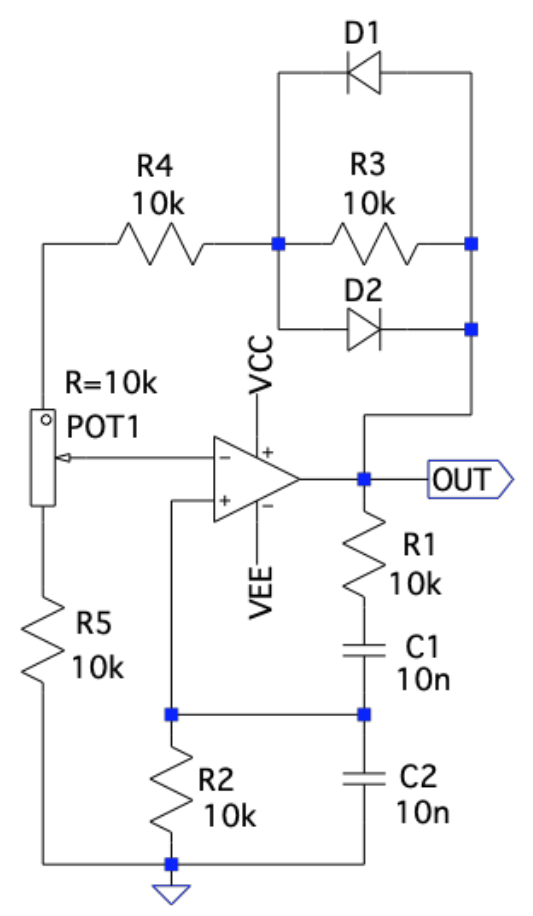
\includegraphics[width=0.4\linewidth]{circuitooscillatoreponteWien.png}
    \caption{\small Circuito per la misura del loop-gain.}
    \label{fig:circuitooscillatoreponteWien}
    \end{center}
\end{figure}

\subsection{Analisi dinamica del circuito: Trimmer, Osservazioni e Regolazioni} 

Il segnale in uscita (senza aver variato la posizione del trimmer rispetto al punto precedente) risulta un segnale di terra costante (a meno di rumore).
Muovendo il trimmer, aumentando la parte di resistenza relativa al feedback, è stato possibile innescare l'oscillazione di figura \ref{fig:wienosc1}. Procedendo nello stesso verso con il trimmer si è invece raggiunta la saturazione dell'operazionale (figura \ref{fig:wiensaturazione}).
\begin{figure}[h]
    \begin{center}
    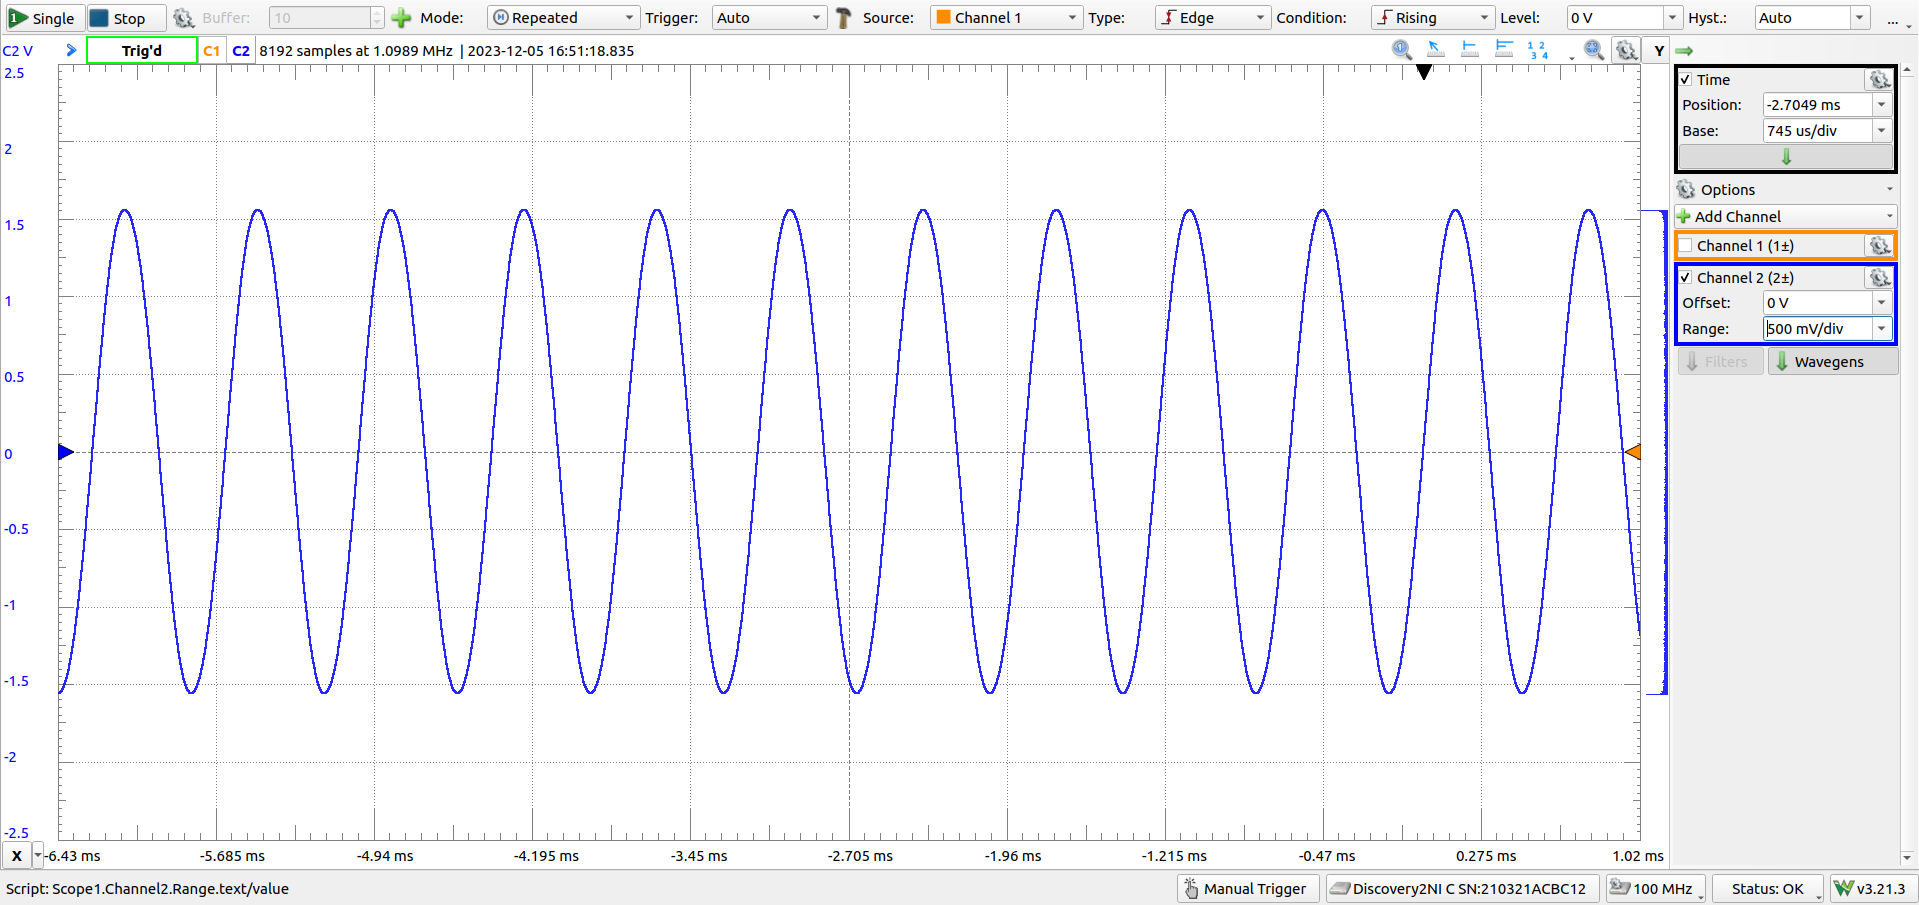
\includegraphics[width=0.7\linewidth]{wienosc1.png}
    \caption{\small Oscillazione del circuito oscillatore a ponte di Wien.}
    \label{fig:wienosc1}
    \end{center}
\end{figure}

\begin{figure}[h]
    \begin{center}
    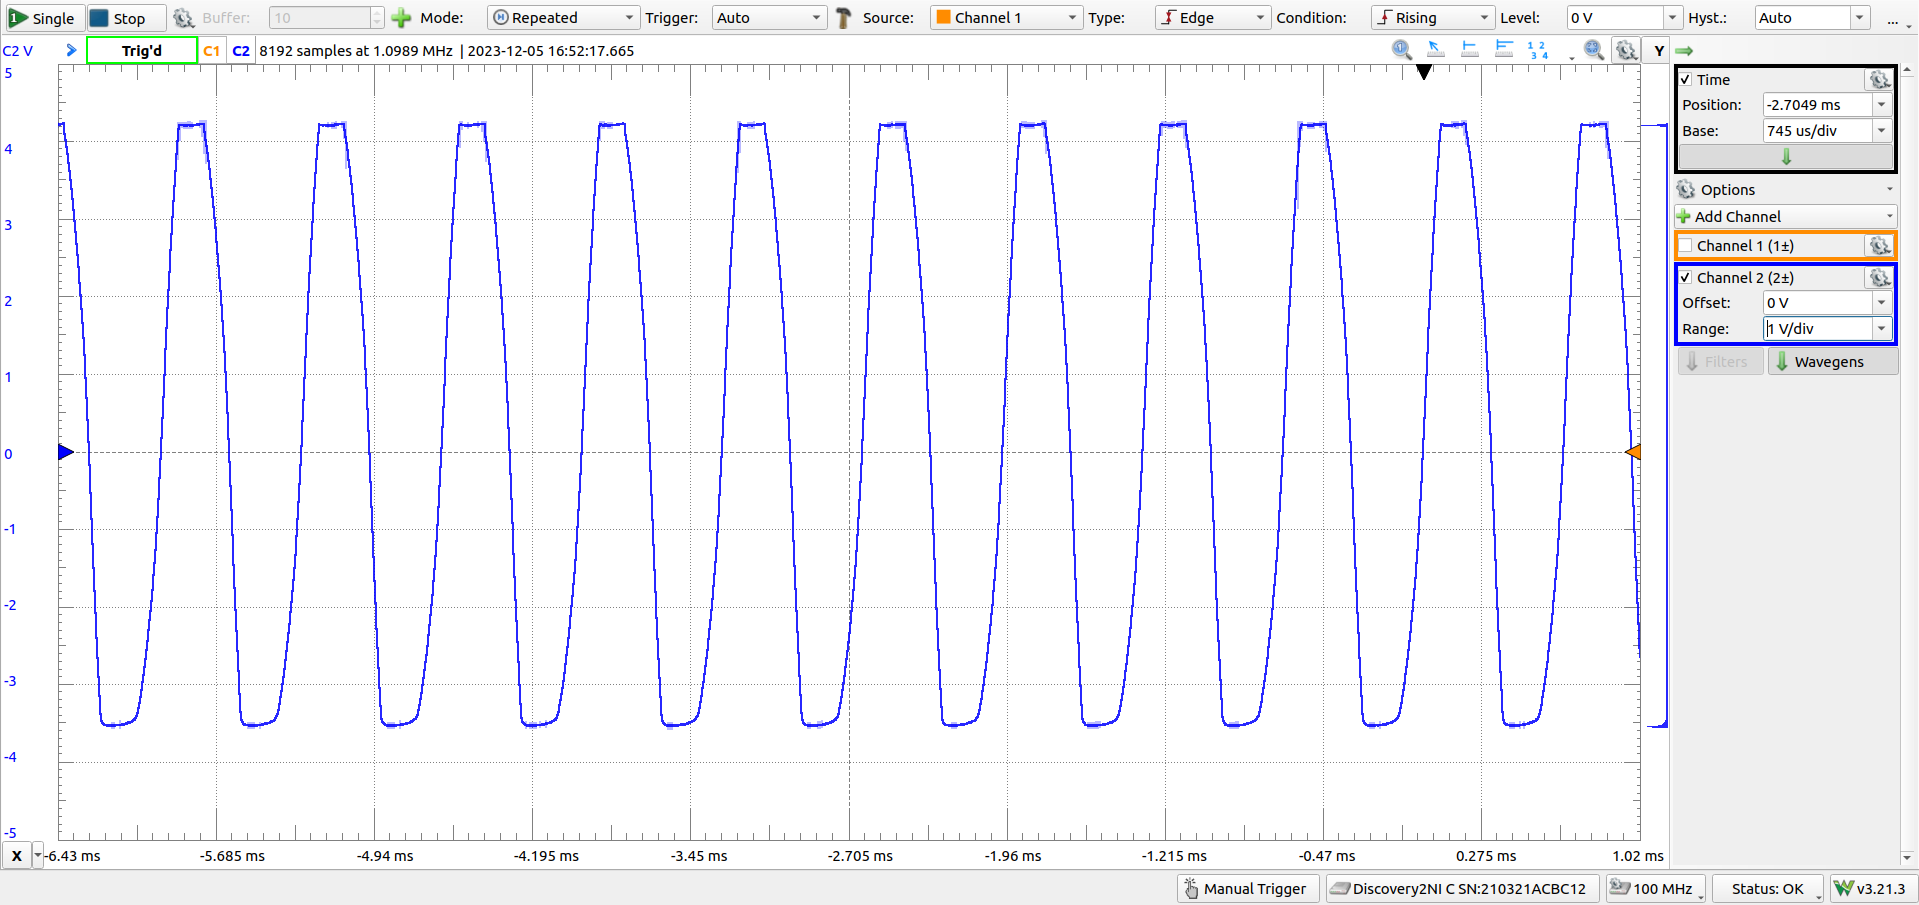
\includegraphics[width=0.7\linewidth]{wiensaturazione.png}
    \caption{\small Oscillazione con saturazione del circuito oscillatore a ponte di Wien.}
    \label{fig:wiensaturazione}
    \end{center}
\end{figure}

Regolata la posizione del trimmer fino
ad osservare l'innesco dell'oscillazione (ma non in saturazione), si ha un'ampiezza di $V_{out} = (1.380 +- 0.005)$ V e un periodo di $T= (627+-3)$ us (figura \ref{fig:wyenperiodo}), il cui errore è stato determinato considerando una distribuzione uniforme, dividendo la grandezza di una singola tacca nel display di misura per $\sqrt{12}$. Da quest'ultimo si ricava una frequenza $f = (1.595+-0.007)$ kHz, compatibile con $f_0$.

\begin{figure}[h]
    \begin{center}
    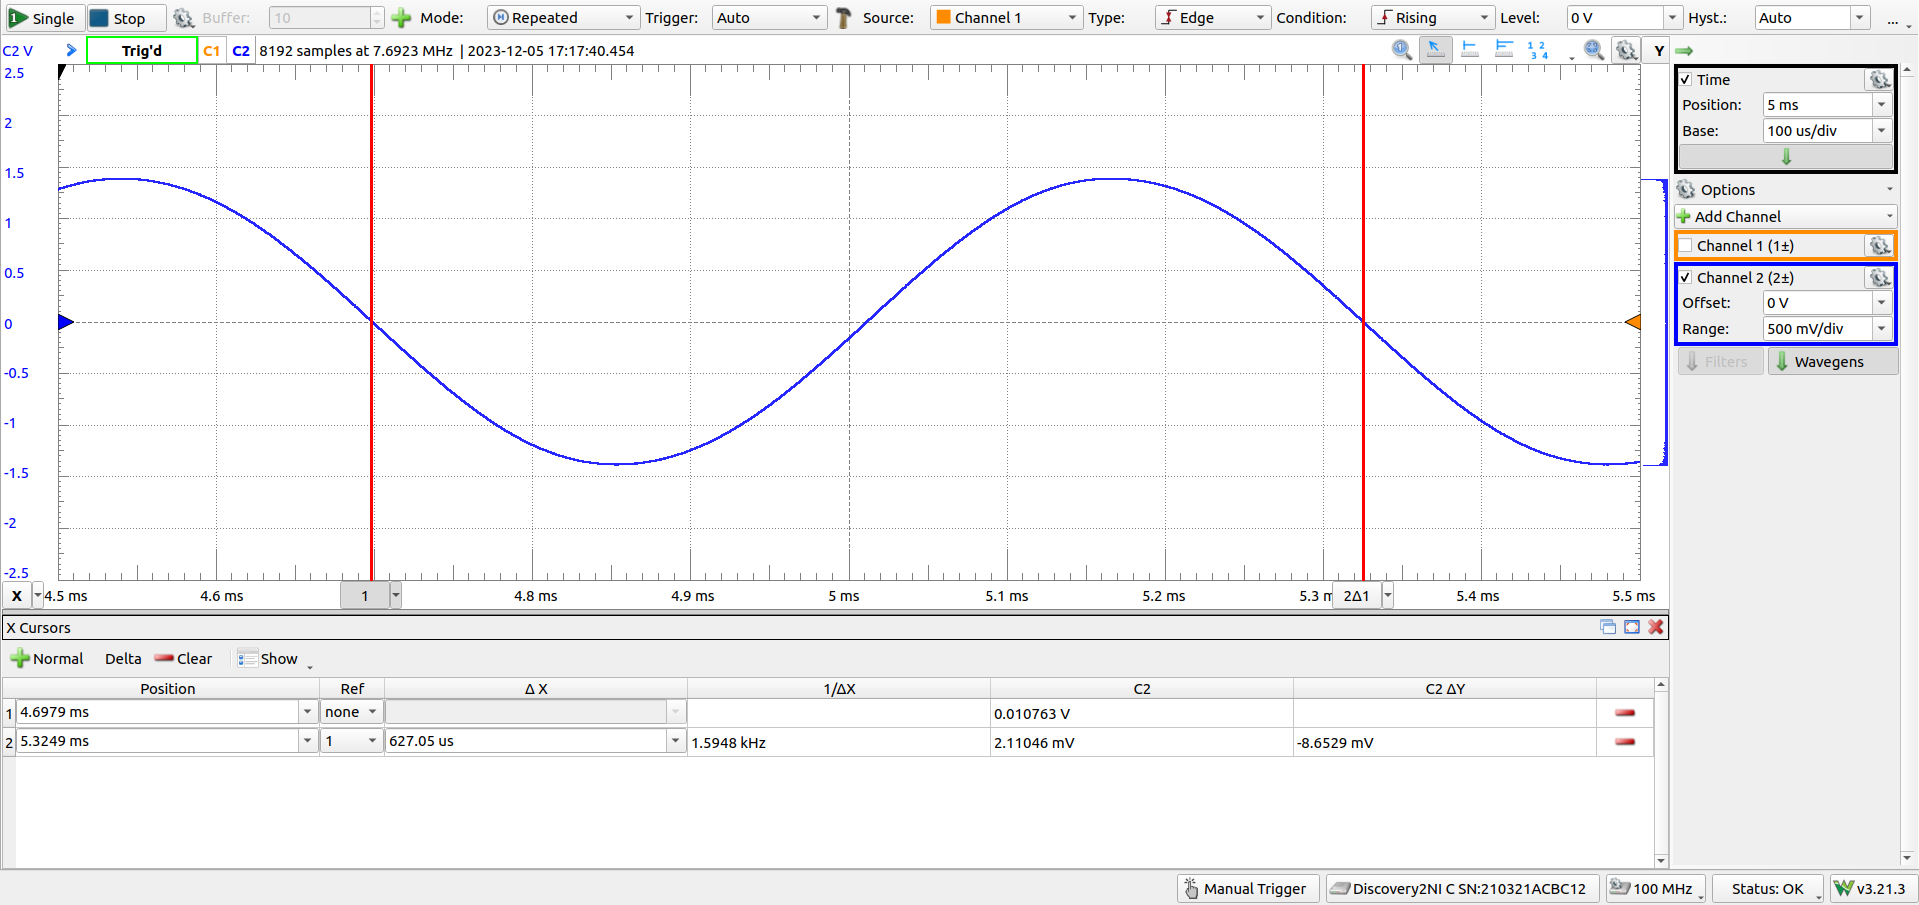
\includegraphics[width=0.7\linewidth]{wyenperiodo.png}
    \caption{\small Misura del periodo dell'oscillazione.}
    \label{fig:wyenperiodo}
    \end{center}
\end{figure}

La forma d'onda di $V_{OUT}$ dall'innesco
dell'oscillazione risulta quella di figura \ref{fig:wieninnesco}
\begin{figure}[h]
    \begin{center}
    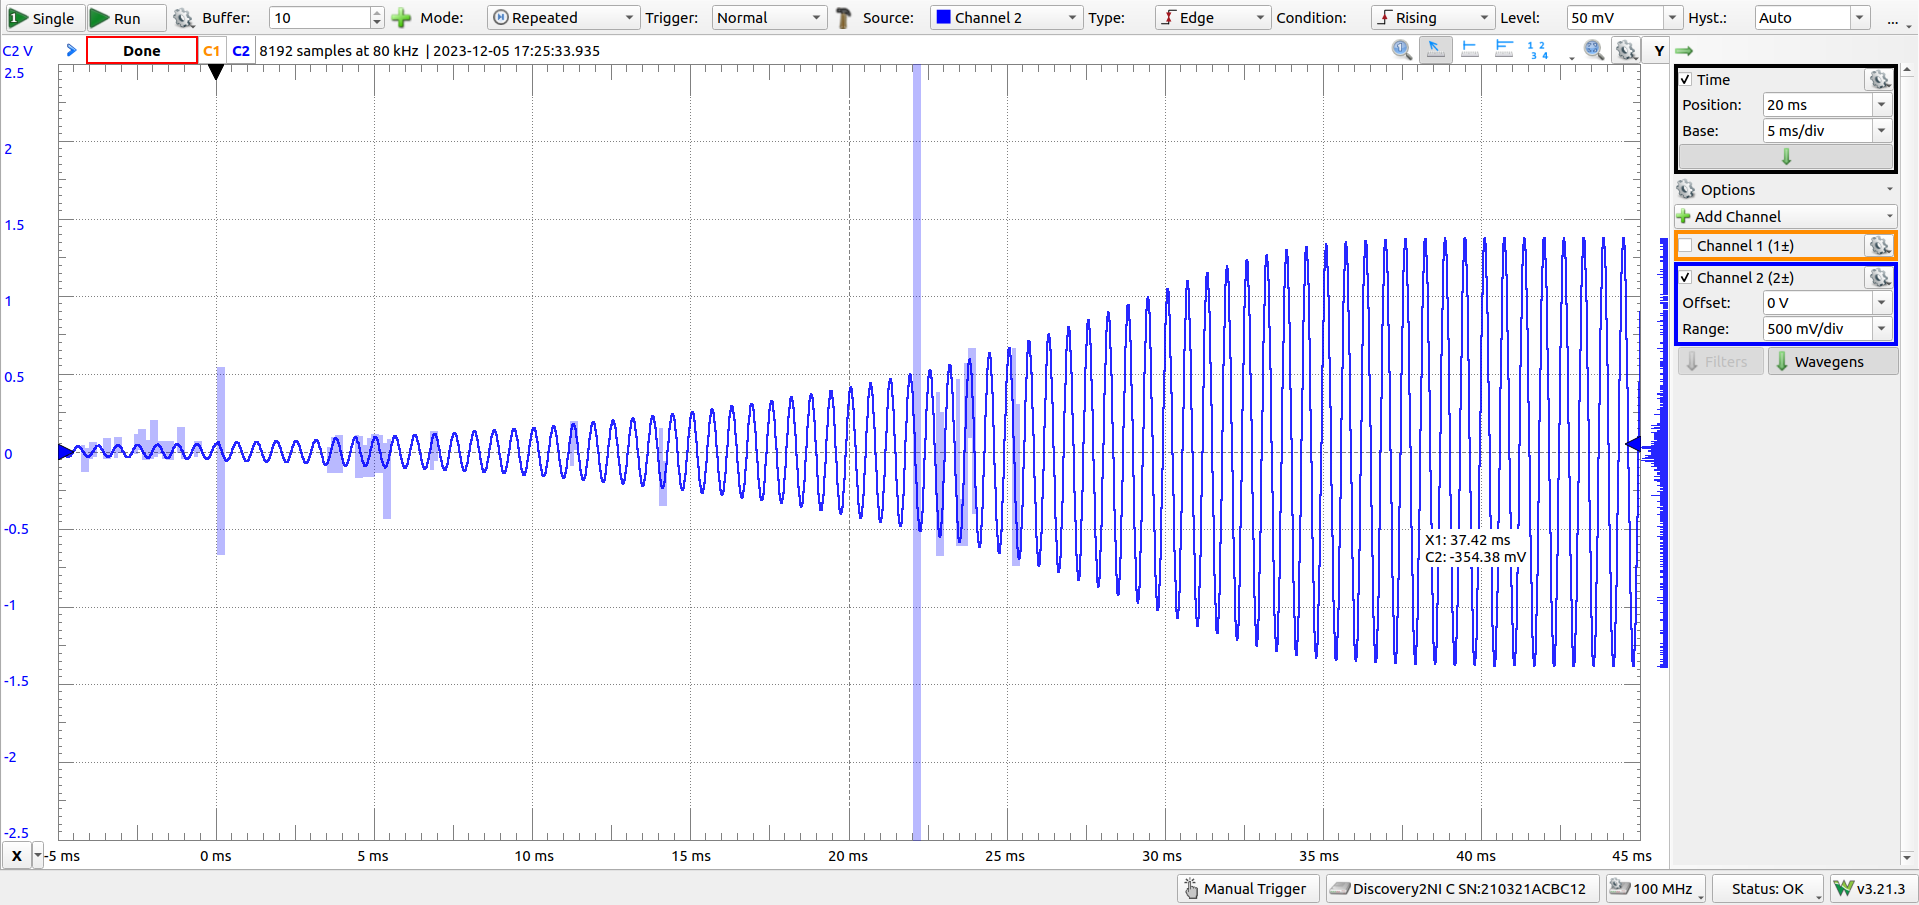
\includegraphics[width=0.7\linewidth]{wieninnesco.png}
    \caption{\small Innesco dell'oscillazione.}
    \label{fig:wieninnesco}
    \end{center}
\end{figure}

Infine, rimuovendo i diodi dal circuito si osserva per $V_{out}$ il comportamento di figura \ref{fig:wiensenzadiodi}. I diodi avevano il ruolo di confinare l'oscillazione in una regione di stabilità, rimuovendoli invece $V_{out}$ raggiunge un'ampiezza elevata di 4 V, sufficiente a toccare i limiti di saturazione, come è evidente dalla figura per le tensioni inferiori.
\begin{figure}[h]
    \begin{center}
    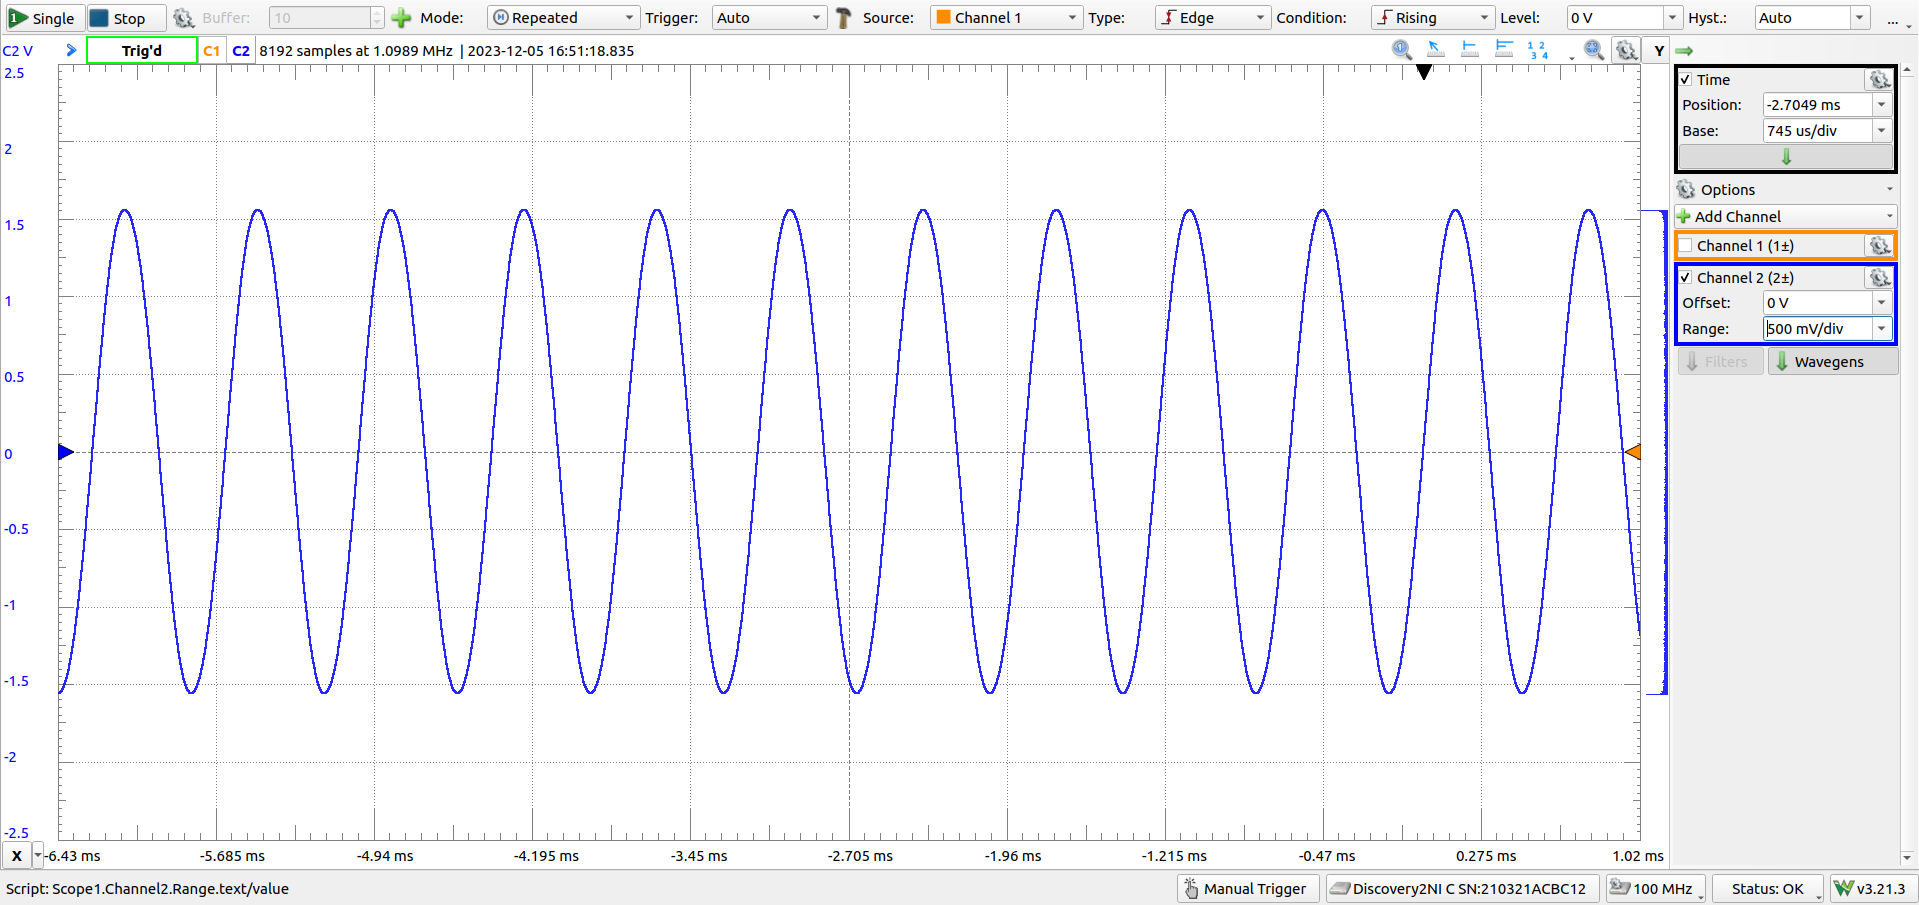
\includegraphics[width=0.7\linewidth]{wienosc1.png}
    \caption{\small Oscillazione con satuzazione inferiore in assenza di diodi.}
    \label{fig:wiensenzadiodi}
    \end{center}
\end{figure}
%%%%%%%%%%%%%%%%%%%%%%%%

\end{document}          
